\documentclass[conference]{IEEEtran}
\IEEEoverridecommandlockouts
\usepackage{cite}
\usepackage{amsmath,amssymb,amsfonts}
\usepackage{algorithmic}
\usepackage{graphicx}
\usepackage{textcomp}
\usepackage{xcolor}
\usepackage{booktabs}
\usepackage{array}
\usepackage{url}
\def\BibTeX{{\rm B\kern-.05em{\sc i\kern-.025em b}\kern-.08em
    T\kern-.1667em\lower.7ex\hbox{E}\kern-.125emX}}
\begin{document}

\title{Design and Empirical Evaluation of a Full-Stack Digital News Portal with an In-Memory Fielded Information Retrieval Engine}

\author{\IEEEauthorblockN{Trieu Nguyen}
\IEEEauthorblockA{\textit{Dept. of Software Engineering, SEG301m Capstone Project} \\
\textit{FPT University}\\
Vietnam \\
trieunguyen2088@gmail.com}
}

\maketitle

\begin{abstract}
Digital news portals require both strict editorial governance and sub-millisecond full-text retrieval across heterogeneous article metadata and prose. Standard relational pattern matching via SQL LIKE or ILIKE degrades rapidly under unstructured news workloads because it performs linear table scans without morphological normalization, field weighting, or probabilistic term-saturation ranking. This paper presents the design and empirical evaluation of a dual-phase full-stack digital news platform that pairs a governed publishing architecture with a custom in-memory Information Retrieval engine. Phase 1 establishes a decoupled three-tier web platform built on Node.js 24 ESM, Express 5, React 19, and PostgreSQL 16 with an 18-table schema managed by 11 idempotent migrations, Argon2id password hashing, rotating HttpOnly refresh token families, RFC 9457 error contracts, and a four-role database-verified RBAC governance matrix. Phase 2 implements an embedded in-memory search engine from first principles, combining a five-phase Porter stemmer, a five-field positional inverted index compressed via Delta and Variable-Byte encoding for a 75.0 percent RAM reduction, skip pointers, Fielded Okapi BM25F, Query Likelihood Dirichlet language modeling, RM3 pseudo-relevance feedback, and K-Means++ result clustering. Across a 16-query evaluation benchmark over 104 Wikinews articles, the primary BM25F ranker achieves 95.00 percent Precision at 5, 0.9228 Mean Average Precision, and 0.226 ms average query latency at 4,418 queries per second, outperforming a Vector Space TF-IDF baseline with statistical significance.
\end{abstract}

\begin{IEEEkeywords}
information retrieval, inverted index, Okapi BM25F, Dirichlet language model, role-based access control, variable-byte compression, digital publishing.
\end{IEEEkeywords}

\section{Introduction}
Modern digital newsrooms operate under two simultaneous engineering pressures: maintaining rigorous editorial access control over content lifecycles while delivering instantaneous, relevance-ranked search across continuously updated article corpora. In many mid-scale web applications, full-text search is initially delegated to relational database predicates such as SQL \texttt{LIKE} or case-insensitive \texttt{ILIKE}. While convenient for exact identifier lookups, substring matching over unstructured news prose exhibits fundamental architectural and algorithmic deficiencies. First, unindexed wildcard predicates force $O(N)$ sequential table scans that scale poorly as article length and archive size grow. Second, Boolean substring matching lacks morphological normalization (e.g., conflating ``investigating'' and ``investigation''), treats headline tokens identically to incidental body mentions, and ignores document-length normalization and term-frequency saturation. Third, returning chronological or binary matches provides no probabilistic ordering, forcing readers to inspect irrelevant articles even when high-signal editorial metadata such as tags and search keywords exist.

Conversely, deploying external distributed search clusters introduces operational overhead, cross-service synchronization lag, and eventual-consistency windows where newly published or moderated articles remain unsearchable or exposed past retraction. For a single-node or vertically scaled newsroom portal, an embedded, memory-resident Information Retrieval (IR) engine synchronized directly with transactional publishing mutations eliminates network serialization overhead and guarantees sub-millisecond query execution without external infrastructure dependencies.

To bridge enterprise governance and classical IR engineering within a unified codebase, this work contributes four primary engineering outcomes:
\begin{enumerate}
\item \textbf{Decoupled Full-Stack Publishing Platform:} A three-tier architecture pairing a React~19 Single-Page Application (SPA) with a Node.js~24 ESM / Express~5 REST backend and PostgreSQL~16 persistence (with automatic embedded PGlite fallback), structured around 18 relational tables across five domains and 11 SHA-256-verified idempotent SQL migrations.
\item \textbf{Defense-in-Depth Security and Four-Role RBAC:} A hardened identity and governance layer combining Argon2id credential hashing, 15-minute ephemeral in-memory JSON Web Tokens (JWTs), 30-day \texttt{HttpOnly} refresh token rotation with \texttt{family\_id} replay revocation, RFC~9457 \texttt{application/problem+json} error contracts, and live database-backed role verification across four distinct editorial roles.
\item \textbf{Compressed In-Memory Fielded IR Engine:} A custom search subsystem featuring a five-phase Porter stemmer, 3-shingle Jaccard near-duplicate detection, a five-field positional inverted index compressed via Delta $d$-gap and Variable-Byte (V-Byte) encoding (achieving a 75.0\% memory footprint reduction), and skip pointers with stride $L = \lfloor\sqrt{P}\rfloor$ ($3.8\times$ fewer posting comparisons).
\item \textbf{Multi-Model Probabilistic Ranking and Empirical Evaluation:} Head-to-head implementation and benchmarking of Fielded Okapi BM25F, Query Likelihood with Dirichlet smoothing, BM25+RM3 pseudo-relevance feedback, Feature-Based Hybrid ranking, and a Vector Space TF-IDF baseline across 104 CC~BY~4.0 Wikinews articles and 16 graded queries, supported by paired significance testing, component ablation, and production search telemetry.
\end{enumerate}

The remainder of this paper is organized as follows. Section~II surveys relevant information retrieval models, text compression structures, and web security standards. Section~III details Phase~1, covering the three-tier topology, relational schema, authentication lifecycle, and RBAC matrix. Section~IV presents Phase~2, detailing linguistic preprocessing, empirical Zipf/Heaps corpus laws, V-Byte index compression, and probabilistic scoring formulations. Section~V reports the 16-query benchmark results, statistical significance, ablation experiments, and automated quality assurance. Section~VI concludes with directions for future work.

\section{Related Work and Theoretical Background}
Foundational ad-hoc retrieval began with Salton et al.'s Vector Space Model (VSM) \cite{b1}, which represents documents and queries as high-dimensional term vectors weighted by Term Frequency--Inverse Document Frequency (TF-IDF) and scored via cosine similarity. Although VSM captures global term rarity, linear term-frequency weighting over-rewards repetitive documents and cannot easily reconcile heterogeneous document zones such as headlines and body text without ad-hoc concatenation.

To address term-frequency saturation and multi-field structure in a principled probabilistic framework, Robertson and Zaragoza formalized Okapi BM25 and its multi-field extension BM25F \cite{b2}. Rather than computing independent per-field BM25 scores—which violates the non-linear concavity of term saturation—BM25F aggregates field-weighted pseudo-term frequencies normalized by field-specific document lengths prior to applying the saturation parameter $k_1$. Alongside probabilistic relevance models, Zhai and Lafferty introduced statistical language modeling for retrieval using Query Likelihood with Bayesian Dirichlet prior smoothing \cite{b3}, which models each document as a unigram multinomial distribution smoothed against background collection statistics via parameter $\mu$. When short user queries suffer from vocabulary mismatch, Lavrenko and Croft's Relevance Model 3 (RM3) \cite{b4} performs pseudo-relevance feedback (PRF) by interpolating the original query model with expansion terms drawn from top-ranked initial documents.

Efficient execution of these rankers relies on classical text normalization and inverted index engineering. Porter's five-phase suffix-stripping algorithm \cite{b5} reduces inflectional and derivational variants to canonical stems without requiring heavyweight morphological dictionaries. As synthesized by Manning, Raghavan, and Sch{\"u}tze \cite{b6}, modern inverted indices compress monotonically increasing document identifier lists into $d$-gaps encoded with byte-aligned Variable-Byte (V-Byte) codes, accelerating conjunctive intersections through skip pointers placed at $\lfloor\sqrt{P}\rfloor$ intervals. Vocabulary growth and term-rank skewness in natural language news corpora are governed by Zipf's rank-frequency law and Heaps' sublinear vocabulary growth law \cite{b7}, which inform memory budgeting for in-memory index structures.

On the web systems engineering side, modern API governance increasingly adopts standardized machine-readable error envelopes defined by RFC~9457 (\textit{Problem Details for HTTP APIs}) \cite{b8}, ensuring predictable client handling without exposing internal stack traces. Credential storage best practices rely on memory-hard key derivation via Argon2id \cite{b9} to resist GPU and ASIC brute-force attacks, while contemporary decoupled portals leverage typed schema validation, SPA routing, and ACID-compliant relational persistence \cite{b10} to maintain strict consistency across editorial workflows.

\section{Phase 1: Full-Stack System Architecture and RBAC Governance}

\subsection{Decoupled Three-Tier Topology}
The platform separates presentation, application logic/retrieval, and durable persistence into three cleanly bounded tiers, illustrated in Fig.~\ref{fig:arch}.

\begin{figure}[htbp]
\centering
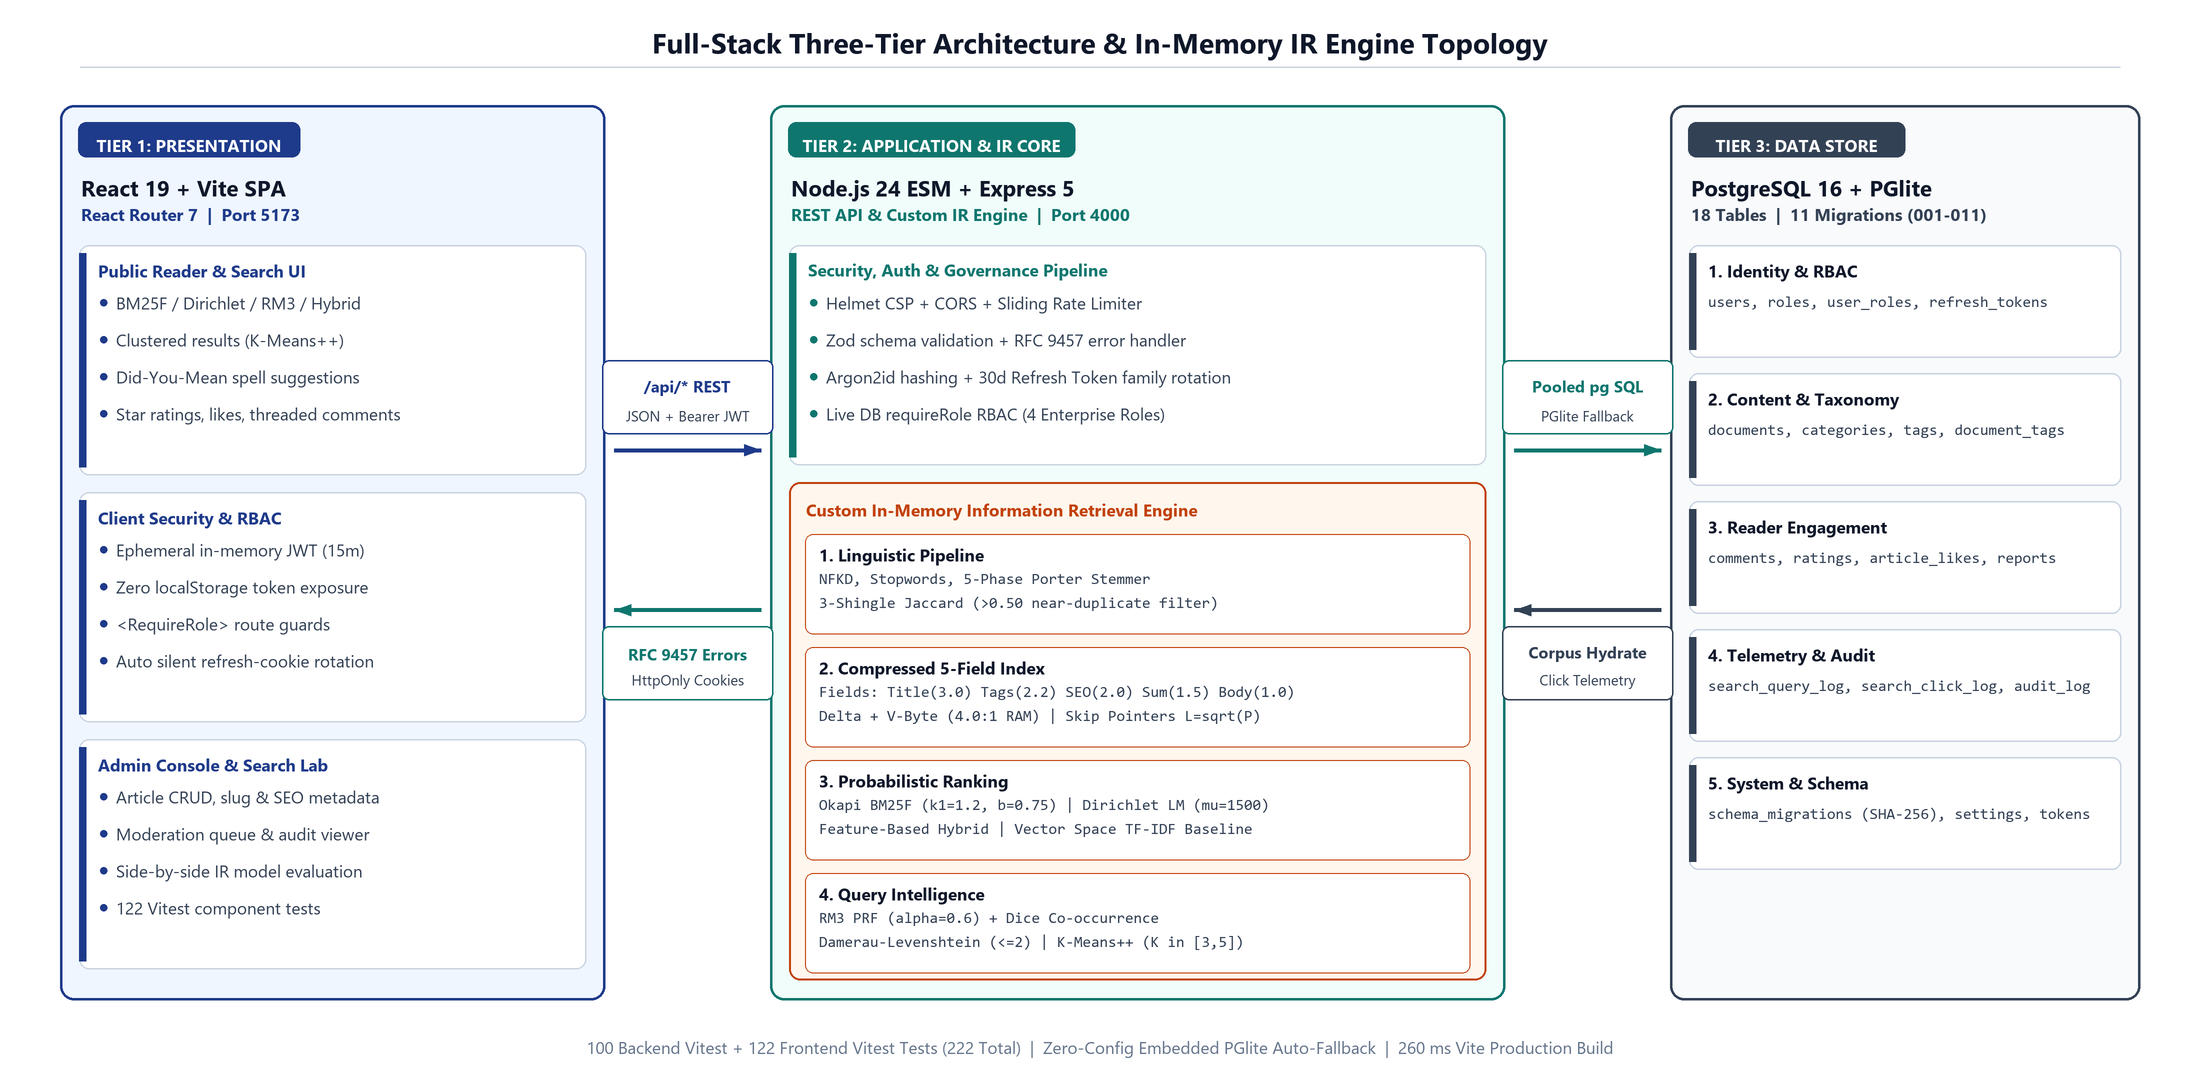
\includegraphics[width=\columnwidth]{fig1_architecture.png}
\caption{Decoupled three-tier system architecture connecting the React~19 SPA (Port~5173), Express~5 API with embedded in-memory IR engine (Port~4000), and PostgreSQL~16 / PGlite persistence layer.}
\label{fig:arch}
\end{figure}

At the presentation tier, a React~19 Single-Page Application built with React Router~7 and bundled via Vite operates on Port~5173. It delivers public news browsing, faceted discovery, interactive search with query suggestions, reader engagement widgets, and role-segmented editorial/administration consoles. At the application tier, a Node.js~24 ECMAScript Module (ESM) backend built on Express~5 runs on Port~4000. All inbound payloads are validated against strict declarative Zod schemas, hardened with Helmet security headers, and routed through centralized error handlers. Crucially, the custom in-memory IR engine executes inside this application tier: it hydrates its compressed inverted index from persisted published documents at startup and processes incremental index updates synchronously upon editorial publication or archival, eliminating cross-network retrieval hops.

At the persistence tier, the backend maintains a connection pool to PostgreSQL~16 for production workloads. To guarantee deterministic zero-configuration execution in local development and automated test suites where an external database daemon may be absent, the database adapter automatically falls back to an embedded WebAssembly PGlite instance while executing identical SQL dialects and migration scripts.

\subsection{Relational Schema and Idempotent Migrations}
Database evolution is governed by 11 sequential SQL migration scripts (\texttt{001} through \texttt{011}). A dedicated \texttt{schema\_migrations} control table records each applied script alongside its cryptographic SHA-256 checksum. On startup, the migration runner verifies checksum integrity against the repository scripts, guaranteeing idempotent execution and halting immediately if previously applied migrations are altered out-of-band.

Across these 11 migrations, the normalized schema comprises 18 relational tables organized into five functional domains:
\begin{itemize}
\item \textbf{Identity and RBAC:} \texttt{users}, \texttt{roles}, \texttt{user\_roles}, and \texttt{refresh\_tokens}, supporting many-to-many role assignments and traceable token rotation lineages.
\item \textbf{Content and Taxonomy:} \texttt{categories}, \texttt{tags}, \texttt{documents}, and \texttt{document\_tags}, storing article headlines, summaries, rich body prose, SEO keywords, publication statuses, and hierarchical/folksonomy labels.
\item \textbf{Community Engagement:} \texttt{comments}, \texttt{ratings}, \texttt{article\_likes}, and \texttt{reports}, capturing reader feedback, 1--5 star evaluations, and content moderation flags.
\item \textbf{Telemetry and Auditing:} \texttt{search\_query\_log}, \texttt{search\_click\_log}, and \texttt{audit\_log}, persisting every executed query, latency, ranker choice, clicked result rank, and privileged administrative mutation.
\item \textbf{System Governance:} \texttt{schema\_migrations} and supporting system configuration/state tables maintaining platform metadata and migration integrity.
\end{itemize}

\subsection{Defense-in-Depth Authentication and Refresh Token Rotation}
Account security enforces defense-in-depth across credential storage, session transport, and error reporting. User passwords are salted and hashed using Argon2id \cite{b9}, mitigating side-channel and GPU cracking threats. Upon authentication, the server issues a short-lived 15-minute access JWT held exclusively in ephemeral React application memory rather than browser \texttt{localStorage} or \texttt{sessionStorage}, preventing persistent token theft via Cross-Site Scripting (XSS).

Long-lived session continuity relies on a 30-day refresh token transmitted via an \texttt{HttpOnly}, \texttt{SameSite} cookie inaccessible to client-side scripts. Each issued refresh token belongs to a tracked \texttt{family\_id} lineage in the \texttt{refresh\_tokens} table. Whenever the client exchanges a refresh cookie for a fresh access JWT, the server atomically rotates the refresh token, invalidating the old token while preserving the shared \texttt{family\_id}. If a previously rotated (consumed) refresh token is replayed—an indicator of cookie theft or session hijacking—the server detects the reuse event and immediately revokes every token sharing that \texttt{family\_id}, forcing re-authentication. All authentication, authorization, and validation failures serialize to RFC~9457 \texttt{application/problem+json} responses \cite{b8}, conveying structured \texttt{type}, \texttt{title}, \texttt{status}, \texttt{detail}, and \texttt{instance} fields without leaking stack traces or database internals.

\subsection{Enterprise Four-Role RBAC Matrix and Community Reader Features}
Authorization is enforced redundantly at both API and UI boundaries. On the server, the \texttt{requireRole} Express middleware queries live role assignments in PostgreSQL on protected routes rather than relying solely on potentially stale JWT claims, ensuring immediate revocation when privileges change. On the client, declarative React \texttt{<RequireRole>} route guards restrict navigation and hide unauthorized administrative controls.

\begin{table}[htbp]
\caption{Enterprise Four-Role RBAC Permission Matrix Across Five Operational Pillars}
\begin{center}
\setlength{\tabcolsep}{3.5pt}
\renewcommand{\arraystretch}{1.15}
\begin{tabular}{@{}lccccc@{}}
\toprule
\textbf{Role} & \textbf{User Mgmt} & \textbf{Publishing} & \textbf{Moderation} & \textbf{SEO/Tel.} & \textbf{Sys./Audit} \\
\midrule
Super Admin & Full & Full & Full & Full & Full \\
Content Manager & -- & Full & Read & Metadata & -- \\
Moderator & -- & Read & Full & -- & Audit Read \\
Data \& SEO Spec. & -- & Read & -- & Full & Telemetry \\
\bottomrule
\end{tabular}
\label{tab:rbac}
\end{center}
\end{table}

Table~\ref{tab:rbac} summarizes the four enterprise roles and their separation of duties across five operational pillars:
\begin{itemize}
\item \textbf{Super Admin:} Holds unrestricted authority over user provisioning, role assignment, editorial overrides, moderation escalation, SEO/telemetry inspection, and system \texttt{audit\_log} review.
\item \textbf{Content Manager:} Owns the editorial publishing lifecycle (drafting, editing, tagging, scheduling, publishing, and archiving documents) plus SEO metadata curation, without access to user privilege escalation.
\item \textbf{Moderator:} Governs community safety by inspecting \texttt{reports} queues, hiding or removing policy-violating \texttt{comments}, and reviewing moderation audit trails.
\item \textbf{Data \& SEO Specialist:} Manages search engine optimization fields (\texttt{seoKeywords}, slugs, summaries), monitors search telemetry (\texttt{search\_query\_log}, \texttt{search\_click\_log}), and evaluates ranking models in the Search Lab without altering editorial prose or user accounts.
\end{itemize}

For general readers, the portal supports authenticated and interactive community participation: 1--5 star article ratings with aggregated averages, one-click article likes (\texttt{article\_likes}), nested threaded comments (\texttt{comments}), collaborative user-submitted tags (\texttt{tags}, \texttt{document\_tags}), and structured violation reporting (\texttt{reports}) routed directly to Moderator queues.
